 \documentclass[9pt,twocolumn,twoside]{osajnl}
\journal{ol}
\setboolean{shortarticle}{true}
\usepackage{pifont}
\usepackage{ulem}

\newcommand{\crossout}[1]{
{\color{red} \sout{#1} } 
}
\newcommand{\add}[1]{
{\color{blue} {#1} } 
}

% version uploaded by Git

\title{Phase and Eigenvalue Correlation in Nonlinear Fourier Transform of Second order Solitons}
\author[1,2*]{Wen Qi Zhang}
%\author[1,2]{Marco Tanner}
\author[1]{Terence Chan}
\author[2]{Shahraam Afshar V.}


\affil[1]{Institute for Telecommunications Research, University of South Australia, Australia}
\affil[2]{Laser Physics and Photonic Devices Laboratories, School of Engineering, University of South Australia, Australia}

\affil[*]{Corresponding author: 
\href{mailto:wenqi.zhang@unisa.edu.au}{wenqi.zhang@unisa.edu.au}}

\begin{abstract}
We investigated the noise correlations in the nonlinear Fourier Transform (NFT) domain for pulses with two eigenvalues. We reduced the 8 degrees of freedom of the pulses to only 4 and show case all NFT parameters (eigenvalues, spectral amplitudes and phases) are correlated, and the correlations are periodic functions of the NFT phase difference with the period of $2\pi$. We also found the maximum correlation always happen at phase difference of 0 or $\pi$. Further study revealed that pulses closely packed eigenvalues behave similar to linear interference and have strong correlation and phase dependency.
\end{abstract}

\setboolean{displaycopyright}{true}

\begin{document}

\maketitle

%==================================================================================
\section{Introduction}
\label{sec:Introduction}
    
Fibre optic communications denote an indisputable impact on human everyday life and lifestyle with increasing demand for data transfer. Consequentially backbone data traffic is estimated to grow 45\% per annum manifesting a difficult task for optical communication technologies to cope with such an immense capacity growth rate \cite{richardson_filling_2010, ellis_approaching_2010, desurvire_capacity_2006}. This is particularly difficult since fibre optic channels reach a fundamental maximum capacity, due to their nonlinear nature \cite{ellis_approaching_2010, desurvire_capacity_2006}, which is well known as the Linear Shannon capacity \cite{shannon_mathematical_1948}. Experiments have been able to approach this nonlinear-capacity-limit within a factor of two impeding further improvements and inevitably leading to what is known as a "Capacity Crunch" \cite{richardson_filling_2010, ellis_approaching_2010, desurvire_capacity_2006, derevyanko_capacity_2016}. 

Unlike traditional systems, originally designed for linear wireless and wired transmission channels, a novel approach widely known as nonlinear Fourier transform (NFT) aspires to exploit these nonlinearities \cite{Agrawal2006, derevyanko_capacity_2016, essiambre_capacity_2010}. Under NFT a signal $q(t)$ in time domain transforms into a continuous, $Q^c(\lambda)$, and a discrete, $Q^d(\lambda_k)$, spectral part, with continuous and discrete eigenvalues $\lambda$, and $\lambda_k$, respectively \cite{yousefi_information_2014}. Albeit the continuous spectrum is related to dispersive waves, the discrete spectrum is physically related to soliton waves \cite{yousefi_information_2014, yousefi_information_2014-1, Agrawal2006}. This special signal family denotes a certain immunity against nonlinear effects and fibre dispersion \cite{Agrawal2006, derevyanko_capacity_2016}. Given these attributes it is not surprising that eigenvalues pose as desirable information carriers which is demonstrated by recent studies \cite{bulow_experimental_2016, aref_experimental_2015, aref_demonstration_2016, gui_alternative_2017, gui_4_2017, hari_multi-eigenvalue_2014, span_time-bandwidth_2017, zhang_correlated_2019}. Although some of these papers proposed the choice of eigenvalue-pairs, the spectral phases were predominantly used to encode data in a QPSK scheme. In the discrete NFT domain, QPSK modulation encodes data on the phase of the NFT spectral components $Q^d(\lambda_k)$ \cite{bulow_experimental_2016, aref_experimental_2015, aref_demonstration_2016, gui_4_2017}. Hence, to improve the proposed modulation schemes it is crucial to have knowledge of NFT noise perturbation on spectral phases and eigenvalues. Correlations among the noise perturbation of eigenvalues in multi-soliton systems and correlation between eigenvalues and their corresponding phases have been recently reported~\cite{zhang_correlated_2019, bulow_experimental_2016}. However, in these work, the aspects of correlation that had been studied are limited to a couple of spectral cases. In this paper, we are going to numerically study the correlation in every degrees of freedom of NFT systems with two eigenvalues.

%==================================================================================
\section{Nonlinear Fourier Transform}
\label{sec:NFT}

In the nonlinear Fourier domain, the nonlinear spectra of a signal pulse propagate as:
\begin{subequations}
    \begin{align}
        Q^{c}(\lambda,z) &= |Q^{c}(\lambda,0)|e^{j[\phi^c(\lambda,0)-4\lambda^2 z]} \text{ ,}\label{eq:propagation-qc}\\
        Q^{d}(\lambda_k,z) &= |Q^{d}(\lambda_k,0)|e^{j[\phi^{d}(\lambda_k,0)-4\lambda_k^2 z]} \text{ ,}\label{eq:propagation-qd}
    \end{align}
\end{subequations}
where $\phi^c(\lambda,0)$ and $\phi^d(\lambda_k,0)$ are the real initial phase of the NFT spectra.

In this work, we focus on the discrete part of the spectrum and use subscripts $Q^d_k$ and $\phi^d_k$ to represent the discrete spectral amplitude associated with the discrete eigenvalue $\lambda_k$. Using Eq. (\ref{eq:propagation-qd}), one can find the NFT spectral amplitude and phase at position $z$ as,
\begin{subequations}
    \begin{align}
        |Q^d_k(z)| &= |Q^{d}(\lambda_k,0)|e^{4\text{Im}(\lambda_k^2)z} \text{ ,}\\
        \phi^d_k(z) &= \phi^d_k(0)-4\text{Re}(\lambda_k^2)z \text{ .}
    \end{align}
\end{subequations}

Considering a pulse with two eigenvalues $\lambda_1$ and $\lambda_2$ propagating along a fibre, due to the differences in $\lambda_1$ and $\lambda_2$, $\phi^d_1$ and $\phi^d_2$ will increase differently as propagation distance increase. We will call this phase difference as the ``\emph{NFT phase difference}" $\Phi$, where
\begin{equation}
    \Phi(z) = \phi^d_1(0)-\phi^d_2(0)-4z(Re(\lambda^2_1)-Re(\lambda^2_2)) \text{.}
    \label{eq:DefNFTphaseDifference}
\end{equation}
or
\begin{equation}
    \Phi(z) = \phi^d_1(0)-\phi^d_2(0)-4z(\lambda^2_1-\lambda^2_2) \text{ ,}
    \label{eq:DefNFTphaseDifferenceIm}
\end{equation}
if $\lambda_1$ and $\lambda_2$ are pure imaginary.

Previously, we discovered that the correlation between eigenvalues in multi-eigenvalue systems are influenced by this phase difference~\cite{zhang_correlated_2019}. And it is also worth mentioning that the phase difference was introduced through propagating the pulse for a distance $z$. 
In particular, when discrete eigenvalues are pure imaginary, 
Eq.\ref{eq:DefNFTphaseDifferenceIm} indicates that in the NFT domain, propagating a pulse is equivalent to change its initial NFT phase. Nevertheless, the NFT spectral correlation was not fully studied. In this work, we are going to explore the correlation in a larger parameter space in the hope of finding out the underlying physics.

%==================================================================================
\section{NFT Correlations}
\label{sec:NFTSpectralCovariances}
Optical solitons are pulses with discrete eigenvalues. To study the "correlation" between eigenvalues and the spectral points associated with the eigenvalues, we will focus on two-eigenvalue solitons in this paper, and through which one will understand NFT better in a broader scale.

In our previous work~\cite{zhang_correlated_2019}, we notice that correlation of the imaginary part of the eigenvalues of a collection of $2sech(t)$ pulses change periodically as the pulse propagates along a fibre. When noises added to the soliton, the eigenvalues and the spectrum will be perturbed. As an example, Figure \ref{fig:fig1} illustrates the scatter plots of noise in $\lambda_1$ and $\lambda_2$ of the $2sech(t)$ pulses at different $\Phi$,
\begin{figure}[htbp]
    \centering
    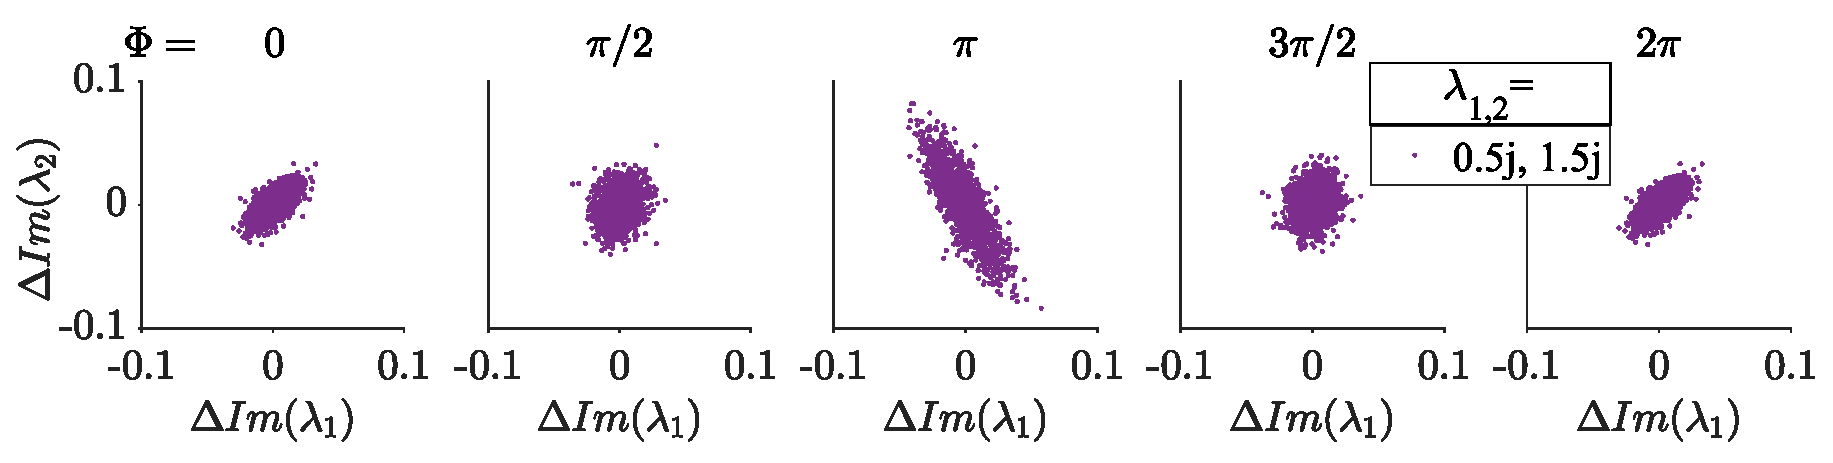
\includegraphics[width=\linewidth]{Fig0_}
    \caption{Noises in eigenvalues when white noises are added to $2sech(t)$ pulses (two eigenvalues at $0.5j$ and $1.5j$) with different phase difference $\Phi$ induced by propagation.}
    \label{fig:fig1}
\end{figure}
in which we define $\Delta Im(\lambda_k)=Im(\lambda_k)-Im(\overline{\lambda_k})$, where $\overline{\lambda_k}$ is the mean of $\lambda_k$. Each scatter plot corresponds to a covariance matrix $\Lambda$ shown as,
\begin{equation}
    \Lambda\Big(A,B\Big)=
    \begin{bmatrix} 
        var(A) & cov(A,B)\\
        cov(B,A) & var(B)
    \end{bmatrix}\text{ ,}
    \label{eq:CovDefNFTphaseDifference}
\end{equation}
where, in this case, $A=Im(\lambda_1)$, $B=Im(\lambda_2)$, $var(x)$ and $cov(x,y)$ are the variance and covariance function, respectively. Similar covariance matrices can be written for $|Q^d_k|$ and $\phi^d_k$ as well. It is worth to mention that the covariance matrix is defined with respect to a given function $q(t)$ and the additive white Gaussian noise added to $q(t)$.

To quantify the correlation, we consider the correlation coefficient 
\begin{equation}
    \rho_{A,B} = \frac{cov(A,B)}{\sqrt{var(A)}\sqrt{var(B)}}\text{ ,}
    \label{eq:DefCorrCoeff} 
\end{equation}
and to simplify our notation, a two-eigenvalue pulse will be denoted by $q(t) \Leftrightarrow (Q_k^d, \lambda_k, \: k=1,2)$. It is important to note the following properties of NFT, from which all other relations of eigenvalue pairs and spectral amplitudes can be derived.
\begin{itemize}[topsep=0pt,itemsep=0pt,partopsep=0pt,parsep=0pt]
    \label{lst:rules}
    \item[\ding{192}] $\frac{1}{|a|}q(t/a) \Leftrightarrow (Q^d_k,a\lambda_k,\:k=1,2)$
    \item[\ding{193}] $q(t-t_0) \Leftrightarrow (e^{-2j\lambda_k t_0}Q^d_k,\lambda_k,\:k=1,2)$
    \item[\ding{194}] $q(t)e^{j\phi} \Leftrightarrow (Q^d_k e^{-j\phi},\lambda_k,\:k=1,2)$
    \item[\ding{195}] $q(t)e^{-2j\omega t} \Leftrightarrow (Q^d_k,\lambda_k-\omega,\:k=1,2)$
\end{itemize}

Suppose $q^1(t)$ is obtained from $q(t)$ through one of the above four transformations. It turns out that the covariance matrix for $q^1(t)$ can also be obtained directly from the covariance matrix for $q(t)$ as well. To illustrate the idea, suppose that $q^1(t)=q(t-t_o)$. Consider the ensemble of random signals $q(t) + n(t)$ where $n(t)$ is the additive white Gaussian noise added to $q(t)$. Due to that $n(t)$ is stochastic, the discrete eigenvalues and the spectral amplitudes of $q(t)+n(t)$ (denoted by  $(\widetilde{Q}_k^d,\widetilde{\lambda}_k,\:k=1,2)$) will be stochastic as well. Using the transformation properties, the discrete eigenvalues and the spectral amplitudes of $q(t-t_o) + n(t-t_o)$ will be distributed as $(e^{-2j\widetilde{\lambda}_k t_0}\widetilde{Q}_k^d,\widetilde{\lambda}_k,\:k=1,2)$. As the white noise is ``time-shift'' invariant in the sense that stochastic properties of $n(t)$ and $n(t-t_o)$ are equivalent. Hence, the discrete eigenvalues and the spectral amplitudes of $q(t-t_o)+n(t)$ will also be distributed as $(e^{-2j\widetilde{\lambda}_k t_0}\widetilde{Q}_k^d,\widetilde{\lambda}_k,\:k=1,2)$. For that reason, we can determine the covariance matrix for $q(t-t_o)+n(t)$ from that for $q(t)+n(t)$.

A pulse with two discrete eigenvalues have 8 degrees of freedom. They are $Q^d_1$, $Q^d_2$, $\lambda_1$ and $\lambda_2$ (whereas each complex number has two degrees of freedom). However, by invoking properties \ding{192}-\ding{195}, one can ``transform'' it into another two-eigenvalue pulse $\hat{q}(t)\Leftrightarrow (\hat{Q}_k^d,\hat{\lambda}_k,\:k=1,2)$ such that
\begin{itemize}[topsep=0pt,itemsep=0pt,partopsep=0pt,parsep=0pt]
    \item[($i$)] $\hat{Q}_2^d $ is a constant (say equal to $\widetilde{Q}_2$), 
    \item[($ii$)] $\hat{\lambda}_2$ is purely imaginary,
    \item[($iii$)] $Im(\hat{\lambda_1}-\hat{\lambda_2})$ is a fixed constant (say denoted by $\Delta\lambda=j$).
\end{itemize}
Furthermore, if $Re(\lambda_1)=Re(\lambda_2)$ (the case where we are particularly interested in), then $\hat{\lambda}_1$ is also pure imaginary. 

To illustrate the construction, consider a two-eigenvalue pulse $q(t) \Leftrightarrow (Q_1^d,\lambda_1,Q_2^d,\lambda_2)$ where $\lambda_1=x_1+jy_1$ and $\lambda_1=x_2+jy_2$. For simplicity, we assume $x_1=x_2\triangleq\omega$ and $\Delta\lambda=j$. Invoking the properties \ding{192} and\ding{195}, we have
\begin{align}
q^1(t) & \triangleq q(t)e^{-2j\omega t} \Leftrightarrow (Q_1^d,jy_1,Q_2^d,jy_2)   \\ \nonumber
q^2(t) & \triangleq  \frac{1}{|a|}q^1(t/a) \Leftrightarrow (Q_1^d,jay_1,Q_2^d,jay_2) \nonumber
\end{align}
where $a$ is chosen such that $ay_2-ay_1=\Delta\lambda$.

Next, let $t_0={(\text{ln}|\widetilde{Q_2}|-\text{ln}|Q^d_2|})/{(2a y_2 )}$. Then by \ding{193}
\begin{align*}
	q^3(t) \triangleq q^2(t-t_o) \Leftrightarrow \left(Q^d_1\left( \frac{|\widetilde{Q_2}|}{|Q_2^d|}\right)^{y_1/y_2},jay_1,\frac{|\widetilde{Q_2}|Q_2^d}{|Q_2^d|},jay_2\right)
\end{align*}
Finally, let $\phi=\angle{Q_2^d}-\angle\widetilde{Q_2}$ such that $e^{-j\phi}\frac{|\widetilde{Q_2}|Q_2^d}{|Q_2^d|}=\widetilde{Q_2}$. Then by \ding{194}
\begin{align*}
    q^4(t) \triangleq q^3(t)e^{j\phi} \Leftrightarrow \left(e^{-j\phi}Q^d_1\left(\frac{|\widetilde{Q_2}|}{|Q_2^d|}\right)^{y_1/y_2},jay_1,\widetilde{Q_2},jay_2\right).
\end{align*}
As a convention, we often choose $\widetilde{Q}_2=-2j$ and $\Delta\lambda=j$ such that the well known two-eigenvalue pulse $2\text{sech}(t)$ satisfies the three criteria even without any transformation.

Following the discussion above, we conclude that, to demonstrate the correlation properties of two-eigenvalue systems, we will look at $\rho_{Im(\lambda_1),Im(\lambda_2)}$, $\rho_{|Q^d_1|,|Q^d_2|}$ and $\rho_{\phi^d_1,\phi^d_2}$. Due to the reduction by transformations and the assumption that ``component solitons'' have roughly the same frequency range, we assume that $\lambda_1$, $\lambda_2$ are both pure imaginary and their difference is $j$, and $Q_2^d=-2j$. Under the transformation, the remaining degree of freedom is $\lambda_1$, $|Q^d_1|/|Q^d_2|$ and the phase difference $\angle Q^d_1-\angle Q^d_2$. In our simulation, we will consider two cases:
\begin{itemize}[topsep=0pt,itemsep=0pt,partopsep=0pt,parsep=0pt]
	\item  Fix $\lambda_1 = 1.5j$, but vary $|Q^d_1/Q^d_2|$ and $\angle Q^d_1-\angle Q^d_2$.
	\item  Fix $|Q^d_1/Q^d_2|$, but vary $\lambda_1$ and $\angle Q^d_1-\angle Q^d_2$.
\end{itemize}

\subsection{Numerical settings}
To achieve high numerical accuracy, we implemented our own bi-redirection NFT algorithm using a fourth-order Runge-Kutta method. With $2^{14}$ sampling points, we can obtain accuracy more than 10 significant figures for eigenvalues and 8 significant figures for spectral amplitudes. For each pair of eigenvalue and spectral amplitude, a full $2\pi$ range of $\Phi$ is divided into 64 segments. For each segment, 5000 instance of white Gaussian noise were applied to the pulse to obtain statistical results. For the spectral amplitude study, a standard deviation of 0.1 is used for the noise strength and a time window of [-20,20] with $2^{14}$ sampling points are used. For the eigenvalue study, variable standard deviation and time window are used to adapt the pulses but the number of sampling points are kept the same. The rule of thumb for choosing the time window is to ensure pulse amplitudes at the edges of the time windows are smaller than -70 dB with respect to the pulse peak. The choice of noise standard deviation is determined by the smallest eigenvalue and the difference between the eigenvalues such that the noisy eigenvalue clouds never overlap. The pulses were generated using inverse NFT implemented with the Darboux method~\cite{yousefi_information_2014-1} for the given $Q^d_k$ and $\lambda_k$. Gaussian noise were added in the time domain. The pulses were not propagated before being decoded using NFT.

\subsection{Correlation for different spectral amplitudes}
According to property \ding{193}, the NFT spectral amplitude is exponentially proportional to the shift of the pulse in time. Here, we fix $Q^d_2$ to be $-2j$ and vary $|Q^d_1|$ from $6\times10^{-4}$ to $6\times10^4$. The eigenvalues $\lambda_1$ and $\lambda_2$ are fixed to $1.5j$ and $0.5j$ respectively. In this way, we have a familiar case of a $2\text{sech}(t)$ pulse when $Q^d_1=-6j$. The results are shown in Fig.\ref{fig:fig2}, in which the first row shows the pulse in time domain for each combination of $Q^d_1$ and $Q^d_2$ for $\Phi=0$, the second to fourth rows show the correlation coefficients $\rho_{Im(\lambda_1),Im(\lambda_2)}$, $\rho_{|Q^d_1|,|Q^d_2|}$ and $\rho_{\phi^d_1,\phi^d_2}$ as functions of $\Phi$, respectively.
\begin{figure}[htbp]
    \centering
    \includegraphics[width=\linewidth]{QCorrelation}
    \caption{Correlational behaviour of eigenvalues, spectral amplitude and phase as functions of $\Phi$ from $-\pi$ to $\pi$ for varieties of $Q^d_2$ with $Q^d_1$ fixed to $-2j$. The first row shows the pulses in time when $\Phi=0$.}
    \label{fig:fig2}
\end{figure}

The observation of Fig.\ref{fig:fig2} yields following results: 
\begin{itemize}[topsep=0pt,itemsep=0pt,partopsep=0pt,parsep=0pt]
    \item As expected, the part of the pulse corresponding to $[Q^d_1,\lambda_1]$ and $[Q^d_2,\lambda_2]$ separate in time as a logarithmic function of the ratio of $\frac{|Q^d_1|}{|Q^d_2|}$.
    \item Correlation coefficients $\rho_{A,B}$ show patterns of periodic change as functions of $\Phi$. 
    \item High correlation between $Im(\lambda_1)$ and $Im(\lambda_2)$ are observed at $\Phi=0$ and $\pi$ when the two solitons are fully overlapped. When the two solitons separate in time, the eigenvalue correlation reduces and their sensitivity to $\Phi$, defined as $s_{A,B}=max(\rho_{A,B})-min(\rho_{A,B})$, also reduces.
    \item Overall high correlation between $|Q^d_1|$ and $|Q^d_2|$ is also observed when the two solitons are fully overlapped, especially at $\Phi=\pi$. But, when the value of $|Q^d_1|$ becomes larger than value of $|Q^d_2|$, $|Q^d_1|$ and $|Q^d_2|$ become negatively correlated (also most significantly at $\Phi=\pi$) and the overall negative correlation increases for all $\Phi$ as $|Q^d_1|$ increases.
    \item Similar observations can be found in the correlation between $\phi^d_1$ and $\phi^d_2$. 
\end{itemize}
Note that in the first row, the pulses are mirror images of each other in time around $\text{log}_{10}|Q^d_1/6|=0$ (according to property \ding{193} and comparing to $2\text{sech}(t)$ pulse). The pulses for $|Q^d_1|>6$ can be consider the time-reversed pulses for $|Q^d_1|<6$. It is also observed that while the $\rho_{Im(\lambda_1),Im(\lambda_2)}$ is symmetric with respect to $\text{log}_{10}|Q^d_1/6|=0$, but $\rho_{|Q^d_1|,|Q^d_2|}$ and $\rho_{\phi^d_1,\phi^d_2}$ are not symmetric due to the fact that $a(\lambda)$ and $b(\lambda)$ are dependent on the orientation of the pulse in time.

\subsection{Correlation for different eigenvalues}
In this section, we will be looking at correlation for a range of eigenvalues with a fixed difference between $\lambda_1$ and $\lambda_2$. We take $2sech(t)$ pulse as a reference point, for which $\lambda_1=1.5j$, $\lambda_2=0.5j$, $Q^d_1=-6j$ and $Q^d_2=-2j$. We keep the spectral amplitudes and the difference between eigenvalues ($\Delta\lambda=\lambda_1-\lambda_2=j$) constant but vary the eigenvalues logarithmically. The pulses in time domain and correlations of $Im(\lambda_k)$, $|Q^d_k|$ and $\phi^d_k$ as functions of $\Phi$ are shown in Fig.~\ref{fig:fig3}. 

\begin{figure}[htbp]
    \centering
    \includegraphics[width=\linewidth]{LCorrelation}
    \caption{Correlational behaviour of eigenvalues, spectral amplitude and phase as functions of $\Phi$ from $-\pi$ to $\pi$ for varieties of $\lambda_1$ and $\lambda_2$ with a fixed difference of $\Delta\lambda=j$. The first row shows the pulses in time with $\Phi=0$.}
    \label{fig:fig3}
\end{figure}

Similar observations to Fig.\ref{fig:fig2} can be made for eigenvalues smaller than $[1.5j, 0.5j]$. For eigenvalues larger than $[1.5j, 0.5j]$, strong correlations can be found in all aspects of the pulse especially at $\Phi=0$ and $\pi$. As eigenvalues increase, $q(t)$ appear to have two separate pulses in the time domain. Since $\Delta\lambda$ is relatively small comparing to $\lambda_k$, both pulses look similar to the fundamental soliton pulse with eigenvalue $\lambda_k$. However, the time separation in this case is not the same as in the previous section. The separation does not compromise the strength of correlations and their sensitivity to $\Phi$, but rather enhances them. Further investigation reveals that when $\Delta\lambda$ is sufficiently small and when $\Phi=0$, $q(t)$ can be accurately approximated by a linear addition of two fundamental solitons as $q(t)\approx q_l(t)+q_r(t)$, where $q_l(t)$ and $q_r(t)$ correspond to the left and right pulses of $q(t)$, respectively. The eigenvalues and spectral amplitudes of $q_l(t)$ and $q_r(t)$ are 
\begin{subequations}
    \begin{align}
        \lambda_l&=\frac{|Q^d_2|\lambda_1+|Q^d_1|\lambda_2}{|Q^d_1|+|Q^d_2|} & \lambda_r&=\frac{|Q^d_1|\lambda_1+|Q^d_2|\lambda_2}{|Q^d_1|+|Q^d_2|},\\
        |Q^d_l|&=-\frac{|Q^d_1||Q^d_2|}{|Q^d_1|+|Q^d_2|}\frac{\Delta\lambda^2}{(2\lambda_1)^2} & |Q^d_r|&=|Q^d_1|+|Q^d_2|.
    \end{align}
\end{subequations}
The pulses $q_l(t)$ and $q_r(t)$ are generated independently in the time window [-20,20]. Same noise added onto the two pulses does not introduce correlation between their NFT components. However, $\lambda_1$, $\lambda_2$, $|Q^d_1|$ and $|Q^d_2|$ are related through $\lambda_l$, $\lambda_r$, $|Q^d_l|$ and $|Q^d_r|$. Perturbations in either $\lambda_l$, $\lambda_r$, $|Q^d_l|$ and $|Q^d_r|$ will appear simultaneously in $\lambda_1$, $\lambda_2$, $|Q^d_1|$ and $|Q^d_2|$. Hence, the high correlations. The accuracy of the approximation increases as $\Delta\lambda/\lambda_1$ decreases. Therefore, the correlations also increases as $\Delta\lambda/\lambda_1$ decreases.

It is worth mentioning that similar behaviour can be found in multi-eigenvalue systems. $N$ closely separated eigenvalues with the same NFT spectral phase transform into a train of $N$ pulses. This is somewhat similar to a linear Fourier transform. The $N$ pulses are the result of a similar process to interference and hence the high correlations and the high sensitivity to the NFT phase relations among them.

%It is worth mentioning that the relations discovered in this section are related to the layer-peeling property of NFT~\cite{yousefi_information_2014}. However, there is a difference. The pulses mentioned in this section are all supported in the same time windows while the layer-peeling property requires each layer of the pulse being supported by a separate time windows without overlap.

%Further investigation reveals that there is a fundamental difference between the two cases. In the case of Fig.~\ref{fig:fig3}, the value of q(t) between the two peaks is non-zero. In fact, at $\Phi=0$, it is defined by the ratio of $\left|log\frac{|Q^d_1|}{|Q^d_2|}\right|$. When $|Q^d_1|=|Q^d_2|$, $q(t_m)$ reaches the maximum of $2|\Delta\lambda|$, where $t_m$ is the point of minimum $q(t)$ between the two peaks. The left figure of Fig.~\ref{fig:fig4} shows $q(t_m)$ as a function of $\frac{|Q^d_1|}{|Q^d_2|}$. The two peaks are not separable. If one separate the two peaks at $t_m$, the eigenvalues of each individual peaks is not the same as the eigenvalues of two separate solitons, although they are close. On the other hand, in the case of Fig.~\ref{fig:fig2}, the gap between the peaks approaches 0 as $|Q^d_1|$ increases and is shown in the right figure of Fig.~\ref{fig:fig4}. The two peaks in this cases is separable. Each individual peak corresponding to an $[Q^d_k,\lambda^d_k]$ from the original pulse. This is the reason we observe the different correlation behaviors. 
%\begin{figure}[htbp]
%    \centering
%    \includegraphics[width=\linewidth]{Fig4}
%    \caption{The minimum $|q(t)|$ between the two peaks of pulses in the case of Fig.~\ref{fig:fig3} (left) and the case of Fig.~\ref{fig:fig2} (right). $t_m$ is the corresponding time. (left) $|q(t_m)|$ as a function of the ratio of $|Q^d_1|$ and $|Q^d_2|$. (right) $|q(t_m)|$ of pulses with different $|Q^d_1|$ as functions of $\Phi$.}
%    \label{fig:fig4}
%\end{figure}

To summarize, we found the following general rules for correlation of pulses in NFT domain:
\begin{itemize}[topsep=0pt,itemsep=0pt,partopsep=0pt,parsep=0pt]
    \item Correlation coefficients $\rho_{A,B}$ are functions of NFT phase difference $\Phi$ with a period $2\pi$.
    \item The maximum and minimum correlation coefficients can be found at $\Phi=0$ or $\pi$.
    \item The maximum or minimum correlation coefficients exists at $|Q^d_k|$ corresponding to optimum overlap of the two solitons. For instance, $|Q^d_k|=[6,2]$ for $\lambda_k=[1.5j,0.5j]$.
    \item The sensitivity $s_{A,B}$ of the correlation coefficients increases with the reduction of the relative difference between NFT spectral amplitudes and/or the reduction of the relative difference between NFT eigenvalues.
\end{itemize}
%In addition to the general rules, we also discovered that the correlations in spectral amplitude and phase are dependent of the time order of the pulse, i.e., $\rho(q(t))\neq\rho(q(-t))$.

%==================================================================================
\section{Conclusion}
\label{sec:Conclusion}
We have investigated correlations among NFT eigenvalues, spectral amplitudes and spectral phases of systems with two eigenvalues. We have reduced the 8 degrees of freedom (4 of $\lambda_k$, 2 of $Q^d_k$ and 2 of $\phi_k$) to only 4 (by requiring $Q^d_2$ being a constant, $\lambda_2$ being pure imaginary, and $Im(\lambda_2 - \lambda_1)$ being a constant), and showcased numerically the correlation coefficients of $\rho_{Im(\lambda_1),Im(\lambda_2)}$, $\rho_{|Q^d_1|,|Q^d_2|}$ and $\rho_{\phi^d_1,\phi^d_2}$ as functions of $\Phi$. The results revealed that all correlation coefficients are periodic functions of $\Phi$ with a same period of $2\pi$. We also show that the maximum and minimum correlations are located at phase difference of $0$ or $\pi$.

Our results produced a few additional insights into the NFT system: (1) for QPSK and QAM modulations, the temporal order of $q(t)$ directly influence the correlations of its NFT components. $q(t)$ and $q(-t)$ yield different correlation behaviors. (2) A set of closely separated eigenvalues transforms into a train of evenly separated pulses in time. This is similar to a linear Fourier transform. A train of pulses in linear frequency domain transforms into a train of pulses in time domain. The pulse train is considered as the result of interference. In NFT domain, the pulses are also linked though a similar process which results in high correlation and high correlation sensitivity to the NFT phase difference.

The results found in this paper can also be used to improve data encoding on to NFT eigenvalue, amplitude and phase by knowing their expected behaviour and noise perturbation. Although recent studies encoding methods, used in \cite{aref_experimental_2015, bulow_experimental_2016, gui_alternative_2017, gui_4_2017}, already use the absolute NFT phase to encode data in a QPSK or QAM manner, we think conjunct decision making, under consideration of our results will bring further improvement. Furthermore we see big potential in the development of new sophisticated conditional modulation schemes with conjunct decision making on eigenvalues and NFT phases based on our findings, to collaborate data rate improvements in NFT communication systems. 

This research was supported fully by the Australian Government through the Australian Research Council's Discovery Projects funding scheme (project DP190102896).

% Bibliography
\begin{thebibliography}{10}
\newcommand{\enquote}[1]{``#1''}
\bibitem{richardson_filling_2010}
D.~J. Richardson, Science \textbf{330}, 327--328 (2010).

\bibitem{ellis_approaching_2010}
A.~Ellis, {Jian Zhao}, and D.~Cotter, Journal of Lightwave Technology \textbf{28}, 423--433 (2010).

\bibitem{desurvire_capacity_2006}
E.~B. Desurvire, Journal of Lightwave Technology \textbf{24}, 4697--4710 (2006).

\bibitem{shannon_mathematical_1948}
C.~E. Shannon, Bell System Technical Journal \textbf{27}, 379--423 (1948).

\bibitem{derevyanko_capacity_2016}
S.~A. Derevyanko, J.~E. Prilepsky, and S.~K. Turitsyn, Nature Communications \textbf{7}, 12710 (2016).

\bibitem{Agrawal2006}
G.~P. Agrawal, \enquote{Chapter 5 - optical solitons,} in \enquote{Nonlinear
  Fiber Optics (Fourth Edition),} pp. 120 -- 176.

\bibitem{essiambre_capacity_2010}
R.-J. Essiambre, G.~Kramer, P.~J. Winzer, G.~J. Foschini, and B.~Goebel,Journal of Lightwave Technology \textbf{28}, 662--701 (2010).

\bibitem{yousefi_information_2014}
M.~I. Yousefi and F.~R. Kschischang, IEEE Transactions on Information Theory \textbf{60}, 4312--4328
  (2014).

\bibitem{yousefi_information_2014-1}
M.~I. Yousefi and F.~R. Kschischang, IEEE Transactions on Information Theory \textbf{60},
  4346--4369 (2014).

\bibitem{bulow_experimental_2016}
H.~Bülow, V.~Aref, K.~Schuh, and W.~Idler, in \enquote{Optical {Fiber} {Communication} {Conference} (2016),
  paper {Tu}2A.3,}  (Optical Society of America, 2016), p. Tu2A.3.

\bibitem{aref_experimental_2015}
V.~Aref, H.~Bülow, K.~Schuh, and W.~Idler, in \enquote{2015 {European} {Conference} on {Optical} {Communication} ({ECOC}),} (2015), pp. 1--3.

\bibitem{aref_demonstration_2016}
V.~Aref, S.~T. Le, and H.~Buelow, in \enquote{{ECOC} 2016 - {Post} {Deadline} {Paper}; 42nd {European} {Conference} on {Optical} {Communication},} (2016), pp. 1--3.

\bibitem{gui_alternative_2017}
T.~Gui, T.~H. Chan, C.~Lu, A.~P.~T. Lau, and P.~K.~A. Wai, Journal of Lightwave Technology \textbf{35}, 1542--1550 (2017).

\bibitem{gui_4_2017}
T.~Gui, S.~K. Lo, X.~Zhou, X.~Zhou, C.~Lu, A.~P.~T. Lau, and P.~K.~A. Wai, in \enquote{Optical {Fiber} {Communication} {Conference} (2017), paper {Th}2A.58,}  (Optical Society of America, 2017), p. Th2A.58.

\bibitem{hari_multi-eigenvalue_2014}
S.~Hari, F.~Kschischang, and M.~Yousefi, in \enquote{2014 27th {Biennial} {Symposium} on {Communications} ({QBSC}),}  (2014), pp. 92--95.

\bibitem{span_time-bandwidth_2017}
A.~Span, V.~Aref, H.~Bülow, and S.~T. Brink, in \enquote{2017 {IEEE} {International} {Symposium} on {Information} {Theory} ({ISIT}),}  (2017), pp. 61--65.

\bibitem{zhang_correlated_2019}
W.~Q. Zhang, T.~Gui, Q.~Zhang, C.~Lu, T.~M. Monro, T.~H. Chan, A.~P.~T. Lau, and V.~S. Afshar, Scientific Reports \textbf{9}, 6399 (2019).

\end{thebibliography}


% Full bibliography added automatically for Optics Letters submissions; the following line will simply be ignored if submitting to other journals.
% Note that this extra page will not count against page length
\bibliographyfullrefs{references}

% Please include bios and photos of all authors for aop articles
\ifthenelse{\equal{\journalref}{aop}}{%
\section*{Author Biographies}
\begingroup
\setlength\intextsep{0pt}
\begin{minipage}[t][6.3cm][t]{1.0\textwidth} % Adjust height [6.3cm] as required for separation of bio photos.
  \begin{wrapfigure}{L}{0.25\textwidth}
    \includegraphics[width=0.25\textwidth]{john_smith.eps}
  \end{wrapfigure}
  \noindent
  {\bfseries John Smith} received his BSc (Mathematics) in 2000 from The University of Maryland. His research interests include lasers and optics.
\end{minipage}
\begin{minipage}{1.0\textwidth}
  \begin{wrapfigure}{L}{0.25\textwidth}
    \includegraphics[width=0.25\textwidth]{alice_smith.eps}
  \end{wrapfigure}
  \noindent
  {\bfseries Alice Smith} also received her BSc (Mathematics) in 2000 from The University of Maryland. Her research interests also include lasers and optics.
\end{minipage}
\endgroup
}{}


\end{document}
